\section{Student Profiling}
Exploration of datasets as part of the data mining process includes assessing features such as variance and correlation within the data. These features impact the usefulness of datasets in terms of data mining and so are important to quantify during the data exploration phase.

Table \ref{tbl-variance-benchmarks} lists variance measurements for several datasets derived from the admissions data in an effort to assess different means of benchmarking students. These same datasets are tested for correlation with final CSC1015F grade results as shown in Table \ref{tbl-correlation-grades}. An additional dataset is compiled from each benchmarks dataset comprising students change in rank from CSC1015F course grades compared to their class rank in the benchmark dataset. Correlation between this dataset and the events dataset is shown in Table \ref{tbl-correlation-events}.

\begin{table}[H]
    \begin{threeparttable}
        \textbf{Table \ref{tbl-variance-benchmarks}}\par\medskip\par\medskip
        \caption{Variance and Std. Deviation of different possible metrics for benchmarking students during admissions}
        \label{tbl-variance-benchmarks}
        \begin{tabularx}{\textwidth}{>{\hsize=1.6\hsize}X>{\hsize=0.7\hsize}Y>{\hsize=0.7\hsize}Y}
            \toprule
            \mC{c}{Benchmark}                      & \mC{c}{$(\sigma_{\overline{x}})^{2}$} & \mC{c}{$\sigma_{\overline{x}}$} \\
            \midrule
            Gr12 Eng \%                            & 56                                    & 7.5                             \\
            Gr12 Sci \%                            & 101.5                                 & 10.1                            \\
            Gr12 Mth \%                            & 68.1                                  & 8.3                             \\
            NBT AL \%                              & 91.2                                  & 9.6                             \\
            NBT QL \%                              & 176.5                                 & 13.3                            \\
            NBT Mth \%                             & 193.8                                 & 13.9                            \\
            Avg Gr12 \%                            & 52.5                                  & 7.2                             \\
            Avg Gr12 \% (Dbl Mth)                  & 53.3                                  & 7.3                             \\
            Avg Gr12 \% (Dbl Mth \& Sci)           & 59                                    & 7.7                             \\
            Avg NBT \%                             & 102.3                                 & 10.1                            \\
            Avg NBT \% (Dbl AL)                    & 89.7                                  & 9.5                             \\
            Avg NBT \% (Dbl QL)                    & 113.8                                 & 10.7                            \\
            Avg NBT \% (Dbl Mth)                   & 113                                   & 10.6                            \\
            Avg NBT \% (Dbl AL/QL)                 & 99.6                                  & 10                              \\
            Avg NBT \% (Dbl AL/Mth)                & 92.3                                  & 9.6                             \\
            Avg NBT \% (Dbl QL/Mth)                & 117.1                                 & 10.8                            \\
            Avg Gr12 \& NBT                        & 59.4                                  & 7.7                             \\
            Avg Gr12 \& NBT (Dbl Gr12 Mth)         & 55.3                                  & 7.4                             \\
            Avg Gr12 \& NBT (Dbl Gr12 Mth  \& Sci) & 59.1                                  & 7.7                             \\
            \bottomrule
        \end{tabularx}
    \end{threeparttable}
\end{table}
\begin{table}[H]
    \begin{threeparttable}
        \textbf{Table \ref{tbl-correlation-grades}}\par\medskip\par\medskip
        \caption{Correlation between different benchmarking methods and CSC1015F grades}
        \label{tbl-correlation-grades}
        \begin{tabularx}{\textwidth}{>{\hsize=1.3\hsize}X>{\hsize=0.7\hsize}Y}
            \toprule
            \mC{c}{Benchmark}                     & \mC{c}{$r$} \\
            \midrule
            Gr12 Eng \%                           & 0.287       \\
            Gr12 Sci \%                           & 0.465       \\
            Gr12 Mth \%                           & 0.447       \\
            NBT AL \%                             & 0.368       \\
            NBT QL \%                             & 0.533       \\
            NBT Mth \%                            & 0.510       \\
            Avg Gr12 \%                           & 0.485       \\
            Avg Gr12 \% (Dbl Mth)                 & 0.487       \\
            Avg Gr12 \% (Dbl Mth \& Sci)          & 0.493       \\
            Avg NBT \%                            & 0.583       \\
            Avg NBT \% (Dbl AL)                   & 0.559       \\
            Avg NBT \% (Dbl QL)                   & 0.580       \\
            Avg NBT \% (Dbl Mth)                  & 0.583       \\
            Avg NBT \% (Dbl AL/QL)                & 0.567       \\
            Avg NBT \% (Dbl AL/Mth)               & 0.570       \\
            Avg NBT \% (Dbl QL/Mth)               & 0.589       \\
            Avg Gr12 \& NBT                       & 0.610       \\
            Avg Gr12 \& NBT (Dbl Gr12 Mth)        & 0.587       \\
            Avg Gr12 \& NBT (Dbl Gr12 Mth \& Sci) & 0.578       \\
            \bottomrule
        \end{tabularx}
    \end{threeparttable}
\end{table}
\begin{table}[H]
    \begin{threeparttable}
        \textbf{Table \ref{tbl-correlation-events}}\par\medskip\par\medskip
        \caption{Correlation Sakai presence and (course class rank - benchmark class rank)}
        \label{tbl-correlation-events}
        \begin{tabularx}{\textwidth}{>{\hsize=1.3\hsize}X>{\hsize=0.7\hsize}Y}
            \toprule
            \mC{c}{Benchmark}                     & \mC{c}{$r$} \\
            \midrule
            Gr12 Eng \%                           & 0.007       \\
            Gr12 Sci \%                           & -0.091      \\
            Gr12 Mth \%                           & -0.038      \\
            NBT AL \%                             & 0.144       \\
            NBT QL \%                             & 0.166       \\
            NBT Mth \%                            & 0.017       \\
            Avg Gr12 \%                           & -0.073      \\
            Avg Gr12 \% (Dbl Mth)                 & -0.070      \\
            Avg Gr12 \% (Dbl Mth \& Sci)          & -0.076      \\
            Avg NBT \%                            & 0.119       \\
            Avg NBT \% (Dbl AL)                   & 0.128       \\
            Avg NBT \% (Dbl QL)                   & 0.138       \\
            Avg NBT \% (Dbl Mth)                  & 0.087       \\
            Avg NBT \% (Dbl AL/QL)                & 0.141       \\
            Avg NBT \% (Dbl AL/Mth)               & 0.120       \\
            Avg NBT \% (Dbl QL/Mth)               & 0.111       \\
            Avg Gr12 \& NBT                       & 0.016       \\
            Avg Gr12 \& NBT (Dbl Gr12 Mth)        & -0.012      \\
            Avg Gr12 \& NBT (Dbl Gr12 Mth \& Sci) & -0.048      \\
            \bottomrule
        \end{tabularx}
    \end{threeparttable}
\end{table}

NBT scores scores have a higher correlation with CSC1015F grades compared to Grade 12 results in general, with the highest correlation between admissions data and CSC1015F results found when an average of all grade 12 results (that are incorporated into this study) and NBT scores is used as a means of benchmarking students. However this means of benchmarking has the smallest variance as a feature, so it seems likely that higher correlation with CSC1015F is highlighting this feature rather than substantiating the usefulness of this benchmarking method.

Two benchmarking methods stand out: using straight \textit{NBT QL} a \textit{NBT Mth} scores as benchmark datasets. These datasets display a relatively high standard deviation in terms of percentages ($> 13\%$) and correlate better with CSC1015F grades than many other benchmarks (with $r = 0.53$ and $r = 0.51$ respectively)

Three scatter plots of grade/benchmark scores are included as a visual representation of the relationship between benchmark variance and correlation: Figure \ref{fig-correlation-gr12eng} shows a plot of \textit{GR12 ENG} benchmark vs CSC1015F scores, \ref{fig-correlation-avg} shows a plot of \textit{Avg Gr12 \& NBT} benchmark vs CSC1015F scores, and \ref{fig-correlation-nbtql} shows a plot of \textit{NBT QL} vs CSC1015F scores.

No correlation is found between student performance and Sakai usage. This is perhaps because the event data doesn't contain a foreign key to the grade entity, and so it is only possible assess the count of presence events for all sites in relation to the CSC1015F site and not usage of the CSC1015F Sakai site specifically. An example of a scatter plot of rank change vs Sakai events count is shown in \ref{fig-delta-rank}.

\begin{figure}[H]
    \centering
    % \begin{mdframed}
    % \centering
    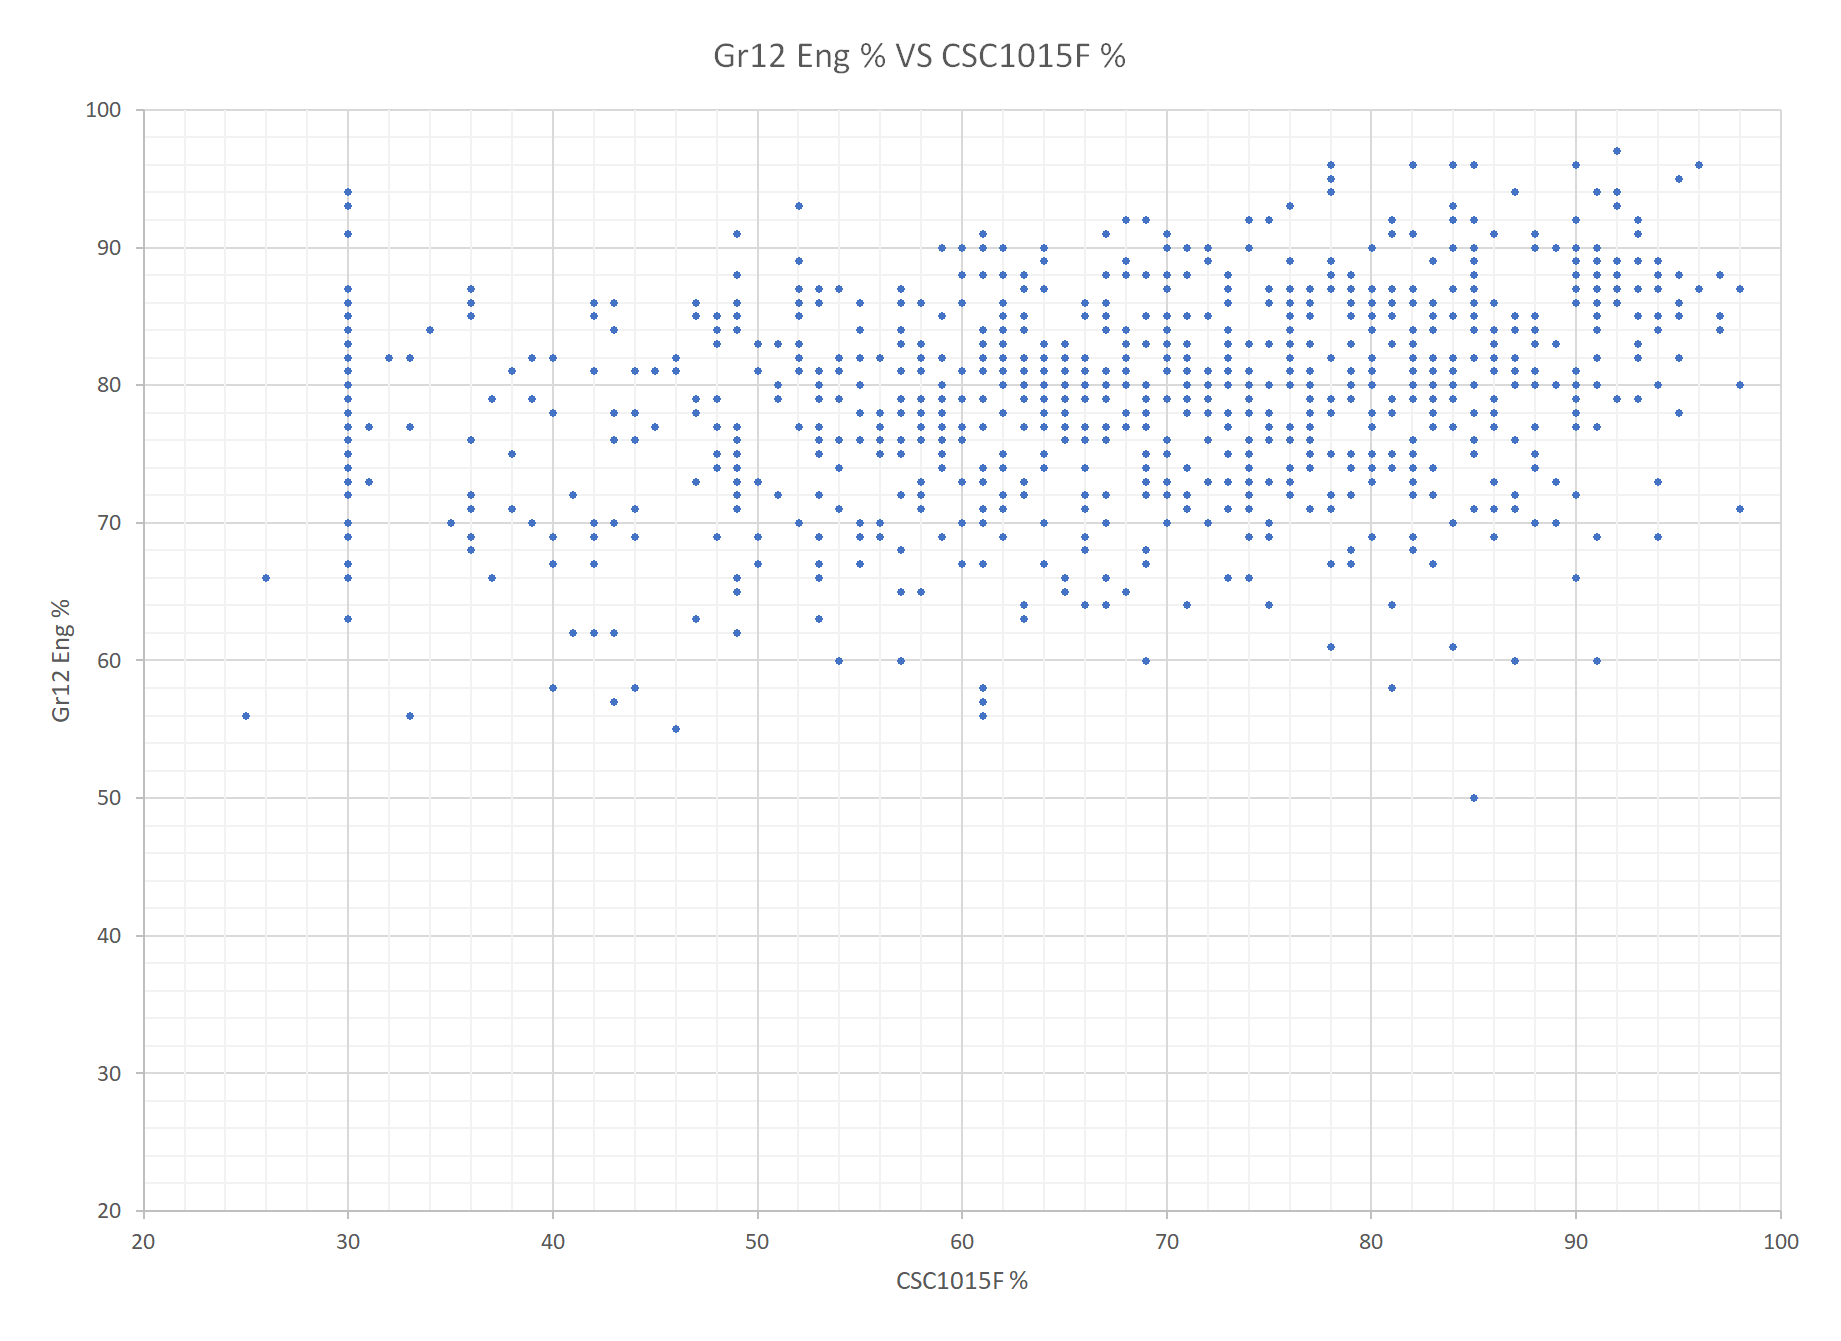
\includegraphics[scale=0.62]{./resources/figures/gr12eng.png}
    % \end{mdframed}
    \caption[CSC1015F \% vs Gr12 Eng \%]{\textbf{Figure \ref{fig-correlation-gr12eng}: CSC1015F \% vs Gr12 Eng \%}}
    \label{fig-correlation-gr12eng}
\end{figure}
\begin{figure}[H]
    \centering
    % \begin{mdframed}
    % \centering
    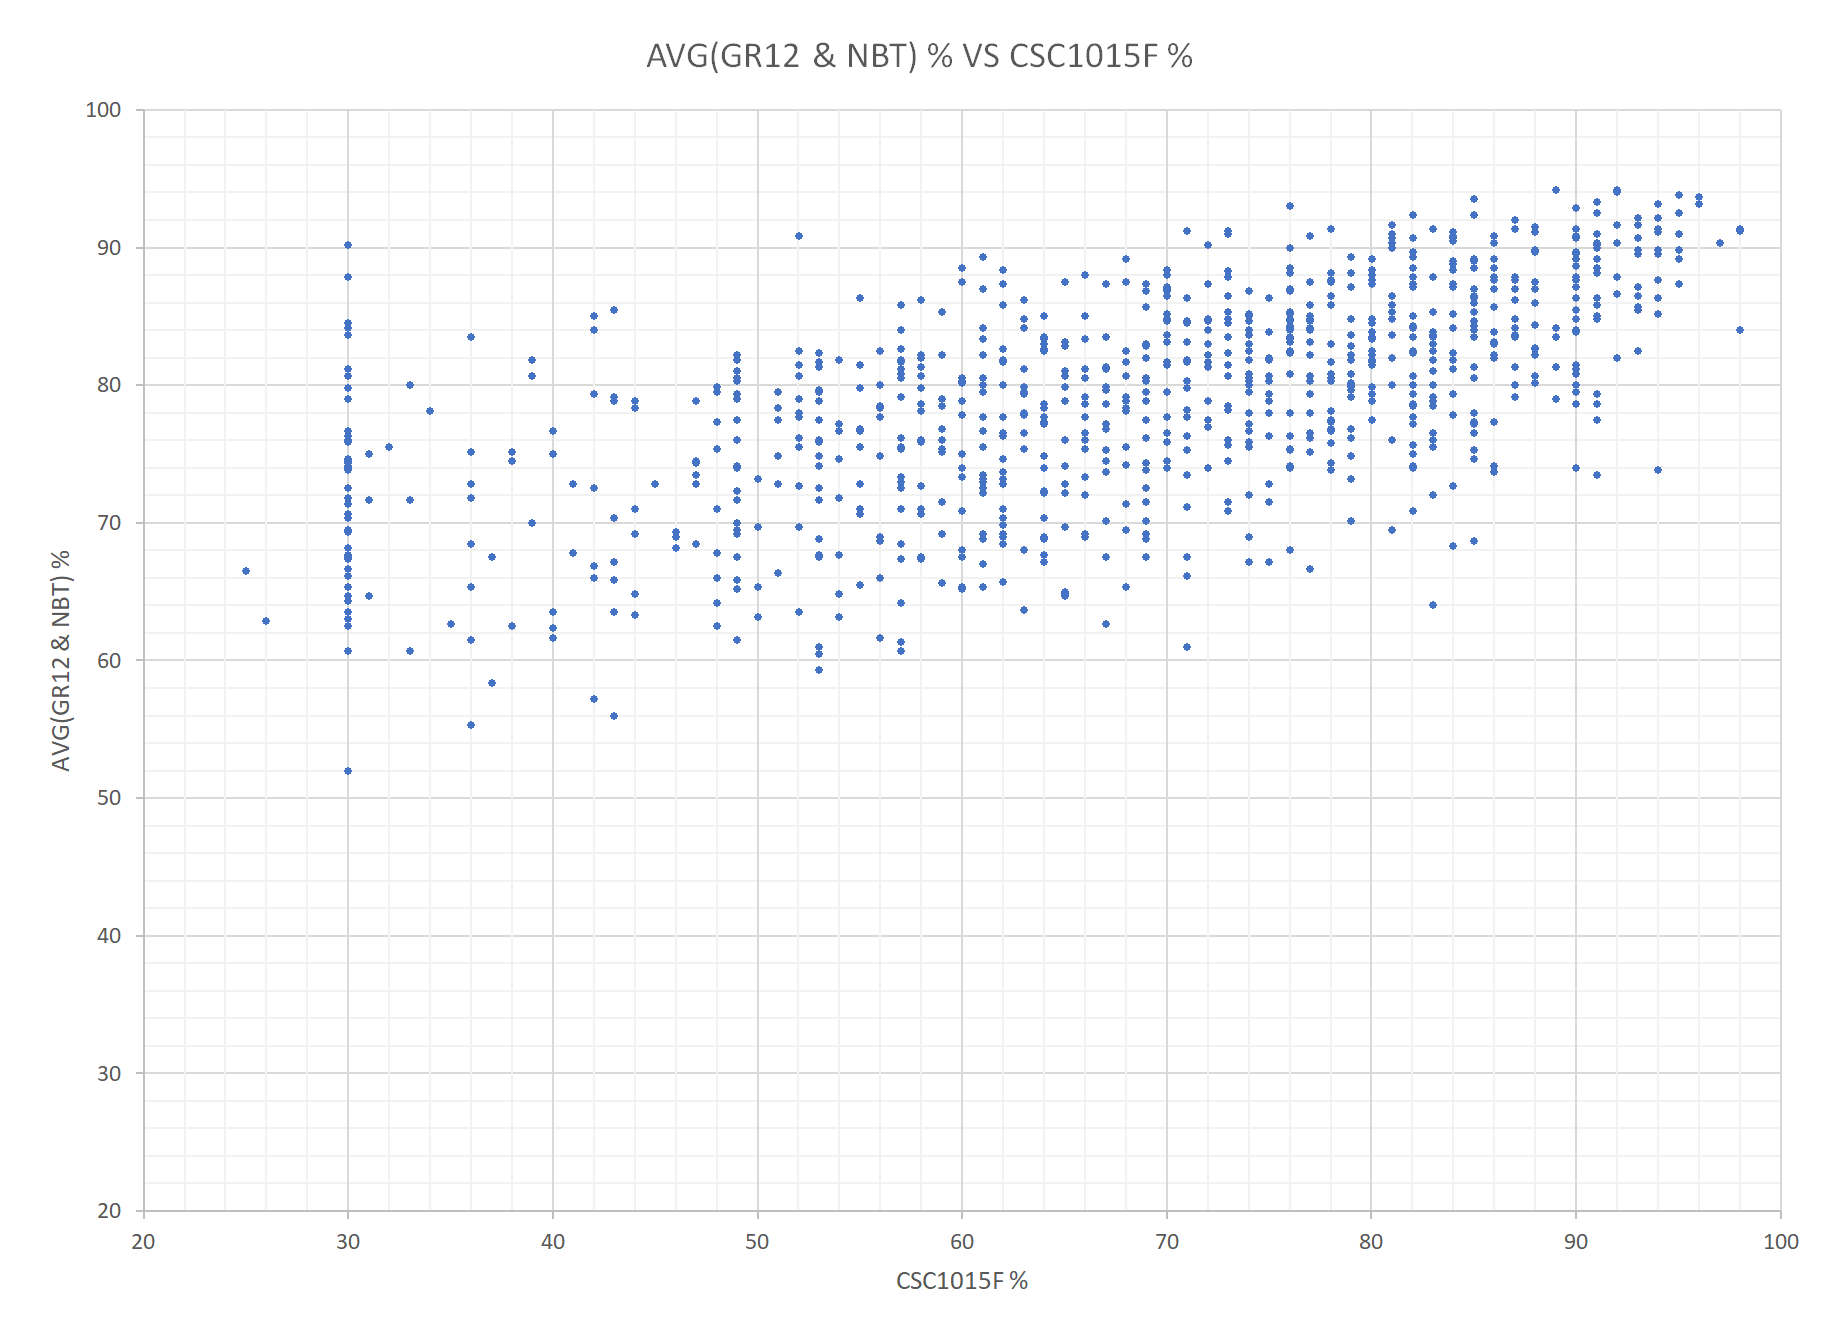
\includegraphics[scale=0.62]{./resources/figures/avg.png}
    % \end{mdframed}
    \caption[CSC1015F \% vs AVG(GR12 \& NBT) \%]{\textbf{Figure \ref{fig-correlation-avg}: CSC1015F \% vs AVG(GR12 \& NBT) \%}}
    \label{fig-correlation-avg}
\end{figure}
\begin{figure}[H]
    \centering
    % \begin{mdframed}
    % \centering
    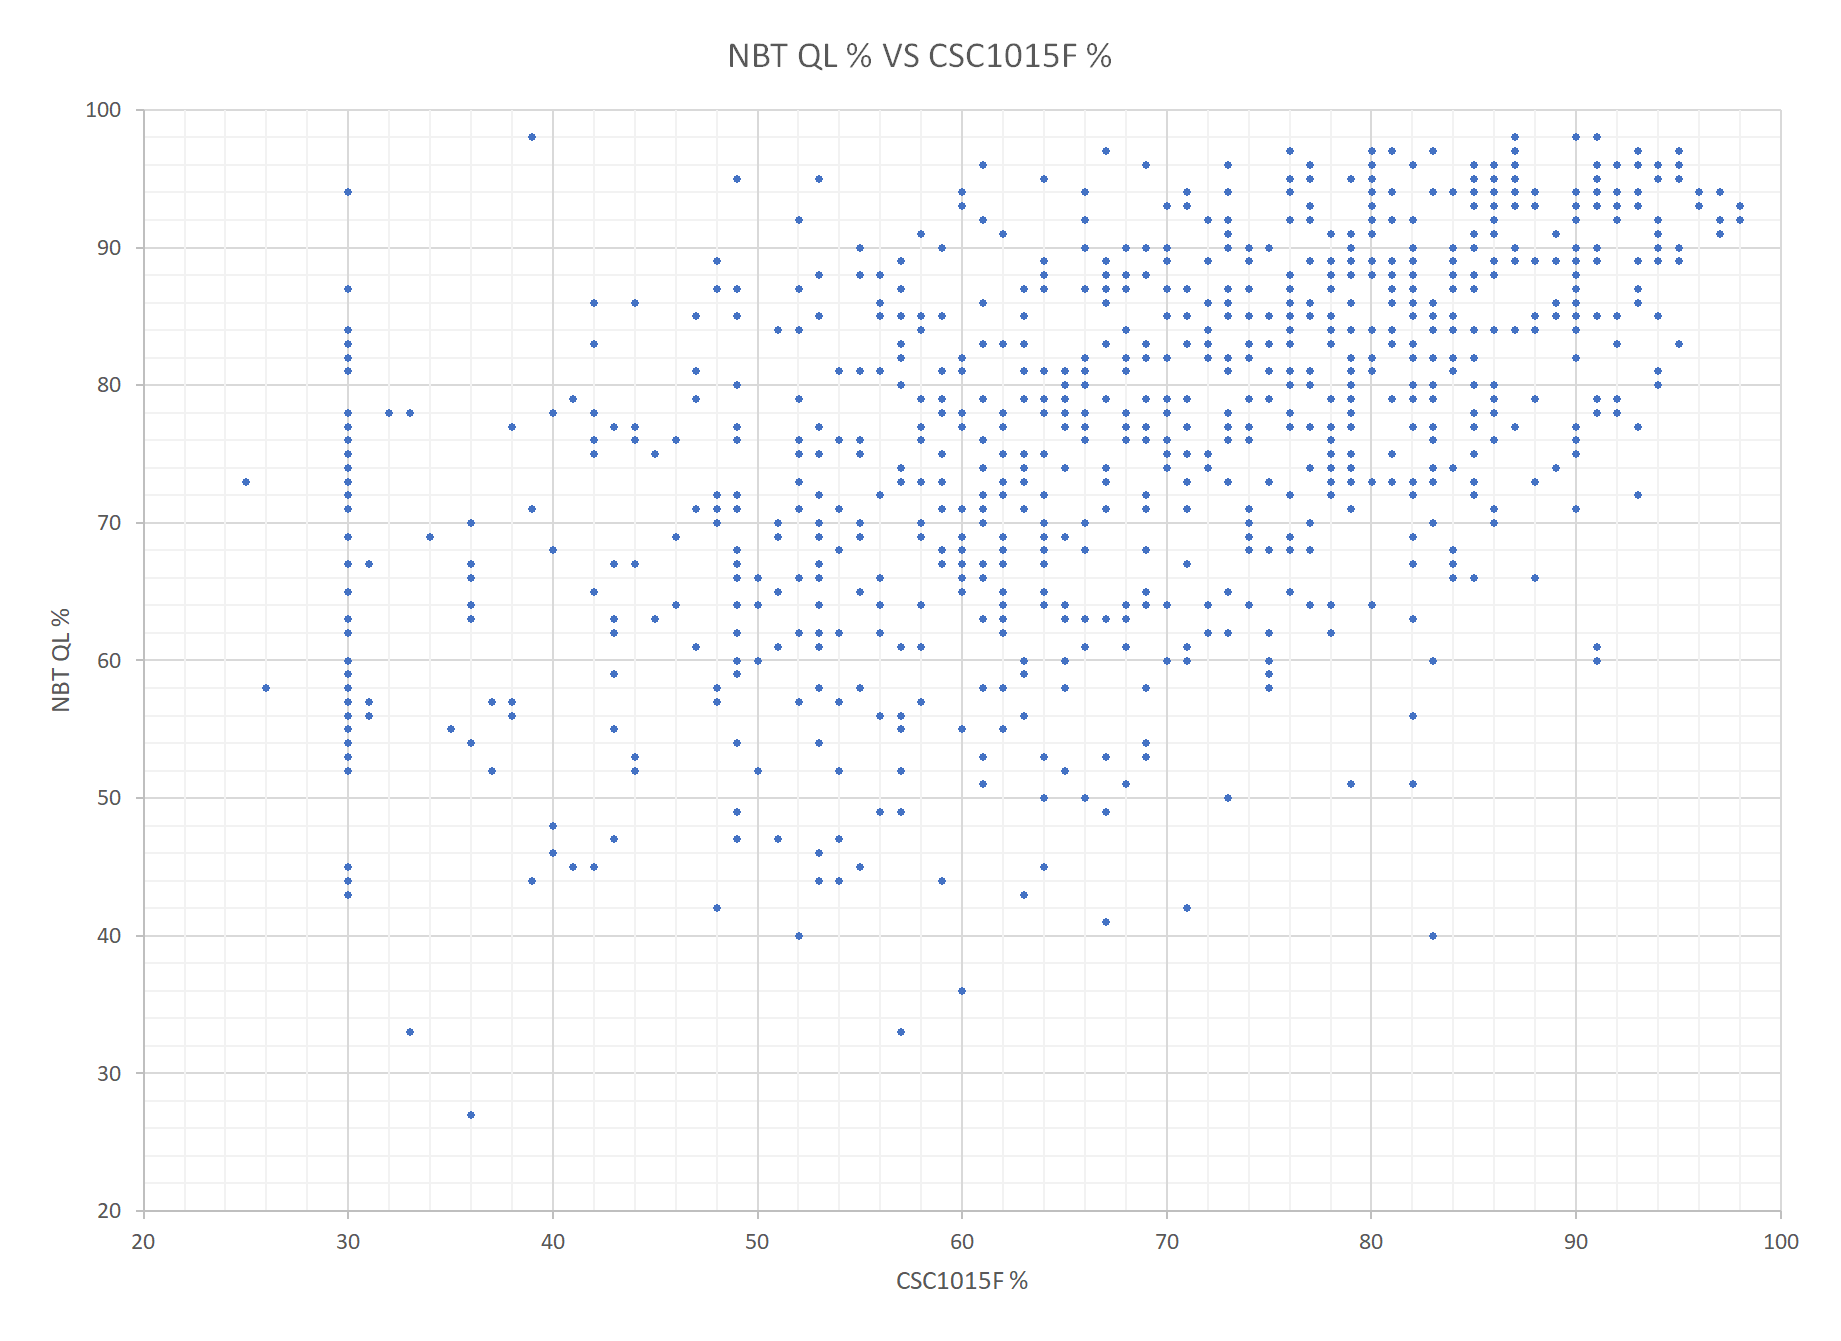
\includegraphics[scale=0.62]{./resources/figures/nbtql.png}
    % \end{mdframed}
    \caption[CSC1015F \% vs NBT QL \%]{\textbf{Figure \ref{fig-correlation-nbtql}: CSC1015F \% vs NBT QL \%}}
    \label{fig-correlation-nbtql}
\end{figure}
\begin{figure}[H]
    \centering
    % \begin{mdframed}
    % \centering
    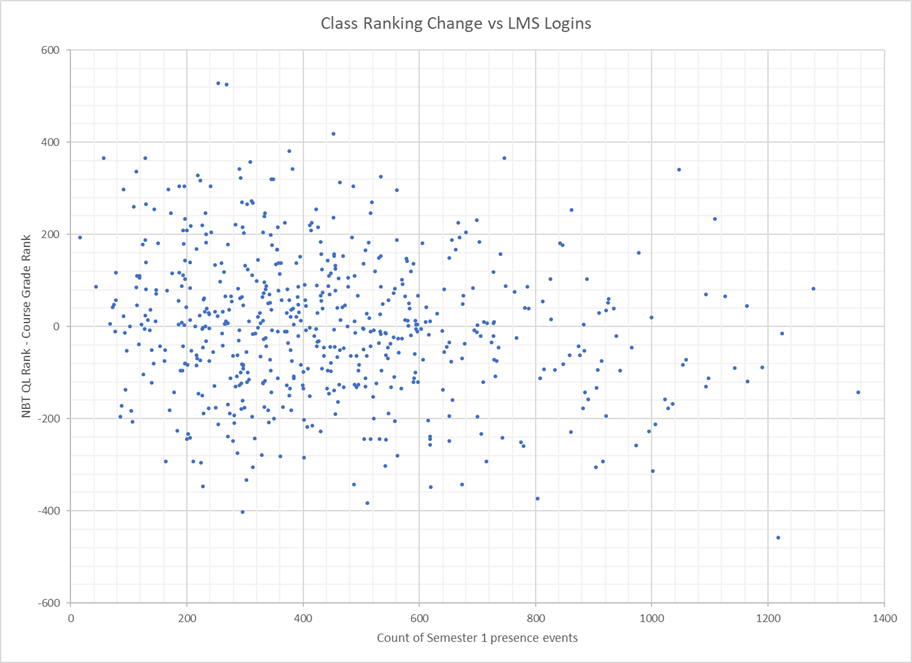
\includegraphics[scale=0.62]{./resources/figures/delta-class-rank.png}
    % \end{mdframed}
    \caption[\( \Delta \) Grade/NBT QL class rank vs Sakai events count]{\textbf{Figure \ref{fig-delta-rank}: \( \Delta \) Grade/NBT QL class rank vs Sakai events count}}
    \label{fig-delta-rank}
\end{figure}